\documentclass[12pt,a4paper]{article}

%########################### Preferences #################################


% ******** vmargin settings *********
\usepackage{vmargin} %This give you full control over the used page arae, it maybe not the idea od Latex to do so, but I wanted to reduce to amount of white space on the page
\setpapersize{A4}
\setmargins{3cm}%			%linker Rand, left edge
		   {1.5cm}%     %oberer Rand, top edge
           {14.7cm}%		%Textbreite, text width
           {23.42cm}%   %Texthoehe, text hight
           {14pt}%			%Kopfzeilenhöhe, header hight
           {1cm}%   	  %Kopfzeilenabstand, header distance
           {0pt}%				%Fußzeilenhoehe footer hight
           {2cm}%    	  %Fusszeilenabstand, footer distance

% ********* Font definiton ************
\usepackage{t1enc} % as usual
\usepackage[utf8]{inputenc} % as usual
\usepackage[french]{babel}
\usepackage{makeidx}
\usepackage[titletoc]{appendix}
\usepackage[shortlabels]{enumitem} 
\usepackage{siunitx}
\usepackage{algorithm}
\usepackage[noend]{algpseudocode}
\usepackage{listingsutf8}
\usepackage{csquotes}
\usepackage[table]{xcolor}
\usepackage{xspace}
\usepackage{hyperref}
\usepackage{xparse}
\usepackage{amssymb}
\usepackage{amsfonts}
\usepackage{mathtools, stmaryrd}
\usepackage{amsmath}
\usepackage[T1]{fontenc}
\usepackage[justification=centering]{caption}
\usepackage{multirow}
\usepackage[pdftex]{graphicx} % required to import graphic files
\usepackage{tikz}
\usetikzlibrary{datavisualization}
\usetikzlibrary{babel}
\usepackage{pgfplots}
\pgfplotsset{compat=1.13}
\usetikzlibrary{plotmarks}
\usepackage{tcolorbox}

% ********* Graphics definition *******
\usepackage{eso-pic} % these two are required to add the little picture on top of every page
\usepackage{everyshi} % these two are required to add the little picture on top of every page
\usepackage[colorinlistoftodos,prependcaption,textsize=tiny]{todonotes}

\DeclarePairedDelimiterX{\Iintv}[1]{\llbracket}{\rrbracket}{\iintvargs{#1}}
\NewDocumentCommand{\iintvargs}{>{\SplitArgument{1}{,}}m} {\iintvargsaux#1}
\NewDocumentCommand{\iintvargsaux}{mm} {#1\mkern1.5mu..\mkern1.5mu#2}
\renewcommand{\arraystretch}{1.2}
\algnewcommand\AND{\textbf{and}\xspace}
\algnewcommand\OR{\textbf{or}\xspace}
\newcommand{\BigO}{\mathcal{O}}
\newcommand{\tdots}{\mathinner {\ldotp \ldotp}}
\renewcommand{\appendixname}{Annexe}
\hypersetup{
    colorlinks  = true,
    linkcolor   = black,
    citecolor   = blue,
    urlcolor    = blue,
    linktocpage = false
}

\pagestyle{plain} % on headers or footers on the first page

\makeindex
\begin{document}

\begin{titlepage}
	\centering
	
\includegraphics[width=0.30\textwidth]{logo.png}\par\vspace{1cm}
	{\scshape\LARGE Sorbonne Universit\'e \par}
	\vspace{1cm}
	{\scshape\Large MOGPL\par}
	\vspace{1.5cm}
	{\Large \bfseries Projet :\par}
	{\huge\bfseries Dice battle\par}
	\vspace{2cm}
	{\Large\itshape HUANG Qijia \par HUANG Weiqing\par}
	
	\vfill

% Bottom of the page
	{\large IMA\par}
	{\large Ann\'ee 2019/2020\par}
\end{titlepage}

%\newpage

%%The following loads the picture on top of every page, the numbers in \put() define the position on the page:
%\AddToShipoutPicture{\setlength\unitlength{0.1mm}\put(604,2522){
\includegraphics[width=1.5cm]{logo.jpg}}}

%\pagestyle{cb} % now we want to have headers and footers

\tableofcontents


\newpage

\part*{Introduction}
\addcontentsline{toc}{part}{Introduction}

Ce projet consiste de trouver un strat\'egie optimal du jeu Dice battle. Deux joueurs choisit \'a lancer entre 1 et D d\'es \'a chaque tour et le nombre de points marqu\'e \'a 1 points si l\'un de d\'es au moins tombe sur 1. Dans le cas contraire, c'est le somme de dés. Le but est de atteintre au moins N points.

L'objectifs de ce projet sont la mise en pratique des algorithme ce qu'on a vu dans le cour(programmation lin\'eaire, programmation dynamique etc). Dans le premier temps, on vas \'etudier la probabilité de marquer un certain nombre de points lorsque l'on lance les dés. Dans le deuxi\`eme temps,on vas étudier le cas s\'equentielle, c'est \'a dire que le joueur 1 lance d'abord le d\'es et ensuite joueur 2 lence le d\'es et ainsi suite. Dans le derni\`ere temps, on vas étudier le cas stiultan\'e, donc deux joueurs lancent le dés stimutan\'ement.  



\newpage

\section{Probabiliste}

\subsection{Question 1}
Explique le r\'eccurence:
\begin{equation}\nonumber
Q(d,k)=\sum\limits_{j=2}^{6}\frac{Q(d-1,k-j)}{5}
\end{equation}

\(Q(d,k)\) signifie la probabilit\'e d'obtenir $k$ points en jetant $d$ d\'es sachant qu'aucun dé n'est tomb\'e sur 1. Supposons que on a d\'ej\`a lanc\'e d-1 d\'es, donc on a
\(Q(d-1,k')\) o\'u \(k'\) est le point marqu\'e en jetant $d-1$ d\'es. Pour le $d$ \`eme d\'es, par définition, on a \(\frac{1}{5}\) de chance tomber sur un des valeurs entre  \(\left\{2,3,4,5,6\right\}\). Donc la moyenne de k :

\begin{equation}\nonumber
k=\frac{(k'+2)+(k'+3)+(k'+4)+(k'+5)+(k'+6)}{5}
\end{equation}
On remplace $k'$ par k en ajoutant une variable $j$, donc on a :
\begin{equation}\nonumber
k=\sum\limits_{j=2}^{6}\frac{(k-j)}{5}
\end{equation}
\medskip
Donc on a bien obtenu la récurrence.

\begin{algorithm}
\caption{Probabilite}
\begin{algorithmic}[1]
\Require $d \geq 0$ \AND $k \geq 0$
\Function{P}{$d$: integer, $k$: $k$: integer}
    \If {$k = 0$}
    	\State \Return $1-(\dfrac{5}{6})^{d}$
    \EndIf 
    \If {$((k \geq 2) \quad \AND \quad(k \leq 2d-1))\quad \OR \quad(k \geq 6d)$}
    	\State \Return 0
    \EndIf
    \State \Return $(\frac{5}{6})^{d} \times \Call{Q}{$d$,$k$}$
\EndFunction

\Statex
\Function{Q}{$d$: integer, $k$: integer}
    \If {$k \leq 0 \quad \OR \quad k< 2d \quad \OR \quad k>6d$} 
        \State \Return 0
	\EndIf    
    \If {$d == 1$} 
        \State \Return $\frac{1}{5}$
    \EndIf
    \For{$j=2$ to $6$}
            \State $res \gets $ $res +\Call{Q}{$d-1$, $k-j$}$
    \EndFor
    \State \Return $\dfrac{res}{5}$

\EndFunction
\end{algorithmic}
\end{algorithm}


\section{Variant séquentielle}
\subsection{Stragégie aveugle}
\subsubsection{Question2}
le nombre de d\'es $d^{*}\left(D\right)$ maximisant l'espérance du nombre de points peut \^etre calculé par:
\begin{equation}\nonumber
d^{*}\left(D\right)=\mathop{\arg\max}_{d}4d(\dfrac{5}{6})^d+1-(\dfrac{5}{6})^d
\end{equation}

\subsubsection{Question 3}
Montrer que $d^{*}\left(D\right)$ n'est pas toujour le choix optimal.

Soit un instance de jeu dont $D=10$,$N=100$. On consid\`ere que un moment le point marqué par joueur 1 est 98 et le points marqué par joueur 2 est j et c'est le tour de joueur 1. Donc joueur 1 a le choix entre 1 à 10 d\'es \'a lancer.Le nombre de d\'es $d^{*}\left(D\right)$ maximisant l'esp\'erance du nombre de points est :
\begin{equation}\nonumber
d^{*}\left(10\right)=\mathop{\arg\max}_{d}4d(\dfrac{5}{6})^d+1-(\dfrac{5}{6})^d=6
\end{equation}
Par contre, le choix optimale est $d=1$ car il minimise le probabilité de marquer juste 1 point dans ce tour(Joueur 1 ne peut pas gangner directement dans ce tour s'il marquera 1 point). Donc $d^{*}\left(D\right)$ n'est pas toujour un choix optimal.
\subsection{Programmation dynamic}
\subsubsection{Question 4}
La formule de r\'ecurrence pour calculer l'esp\'erance de gain $EG(i, j)$ en un état $(i, j)$ est :
\begin{equation}\nonumber
EG(i,j)=-\mathop{\min}_{1 \leq d  \leq D}\sum\limits_{k=1}^{6d}E(j,i+k)
\end{equation}
L'initialisation de r\'ecurrence:
\begin{equation*}
\left .EG(i,j) = \begin{cases} 
      1 & \text{si } i \geq N \\
      -1 & \text{si } j \geq N \\
      
   \end{cases} \right.
\end{equation*}
\subsubsection{Question 5}
Le stratégie optimale s'agit de trouver un nombre de d\'es $d$ qui permet de maximiser l'esp\'erance de gain du joueur1 lorsque le joueur1 a marqué i points et le joueur2 a marqué 2 points. Par la question précedent, on a obtenir dans le cas optimal, l'esp\'erance maximale du joueur 1.Donc il suffit de trouver tel valeur $d$ qui proveque ce r\'esultat:  
\begin{equation*}
d^{*}_{i,j}=-\mathop{\arg\min}_{1 \leq d  \leq D}\sum\limits_{k=1}^{6d}E(j,i+k)
\end{equation*}

\subsubsection{Question 6}
Si on supposait que le nombre de points marqué est 0 si on obtient au moins 1 alors notre algorithme peut jamais s'ar\^eter(car la récurrence commencer par $(0,0)$ et s'arrête  soit sur $(100,j)$ soit sur $(i,100)$, comme k peut être 0, il peut s'exécuter infinitivement). Il a donc une difficulté supplémentaire sur la terminaison.

\subsection{Mise en oeuvre}
\subsubsection{Question 7}
\begin{algorithm}
\caption{Stratégie}
\begin{algorithmic}[1]
\Function{Stratégie aveugle}{$i$: integer, $j$:integer $D$: integer $N$:integer}
	\State $res$: $D$ integer tableau filled with $0$   	
   	\For{$d=1$ to $D+1$}
            \State $res[d] \gets $ $4d(\dfrac{5}{6})^d+1-(\dfrac{5}{6})^d$
    \EndFor
    \State \Return argmax $res$
\EndFunction

\Function{Stratégie optimal}{$i$: integer, $j$:integer $D$: integer $N$:integer}
    \State $E$: $N \times N \times 2$ integer matrix filled with $-2$. The first value of E[i][j] is the esperance and the second value is the quantity of dice. 
    \If {$i \geq N$}
    	\State \Return 1,0
    \EndIf
    \If {$j \geq N$}
    	\State \Return 0,0
   	\EndIf
    \If {$E[i][j][0]!=-2$}
    	\State \Return $E[i][j]$    
    \Else
    \State $res_{max} \gets -\infty$
    \State $d_{optimal} \gets 0$
    	\For{$d=1$ to $D+1$}
    			\State $cum \gets $=0
    			\For{$k=1$ to $6d+1$}
    				\If{$i+k \leq N$}
            			\State $cum \gets $ $cum +\Call{P}{$d-1$, $k-j$} \times -1$
            		\Else 
            			\If {$E[j][i+k][0]==-2$}
            				\State $E[j][i+k] \gets \Call{Stratégie optumal}{$j$,$i+k$,$D$,$N$}$
            			\EndIf
            			\State $cum \gets $ $cum +\Call{P}{$d$, $k$} \times E[j][i+k][0]$	
					\EndIf
				\EndFor
				\If{$res_{max} \leq -cum$}
					\State $res_{max} \gets -cum$
					\State $d_{optimale} \gets d$
				\EndIf	    	
    	\EndFor
    \EndIf
    $E[i][j] \gets res_{max},d_{optimal}$
    \State \Return $E[i][j]$
\EndFunction
\end{algorithmic}
\end{algorithm}

\subsubsection{Question8}
\graphicspath{{.}}
\begin{center}
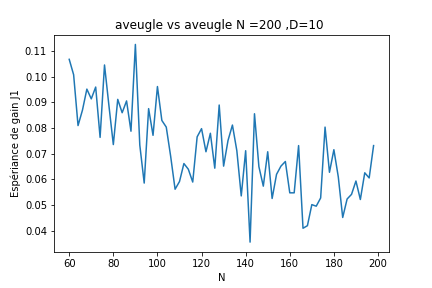
\includegraphics{a_vs_a.png}
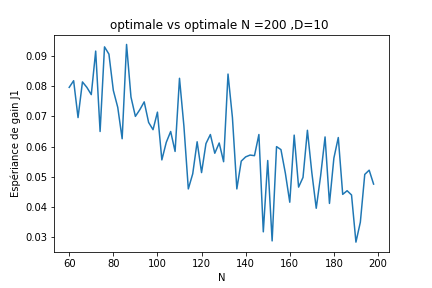
\includegraphics{o_vs_o.png}
\end{center}
On voit que comme le stratégie utilisé pour les deux joueur est le même,plus N est grand,plus l'espérenrance de joueur1 proche de 0 
\begin{center}
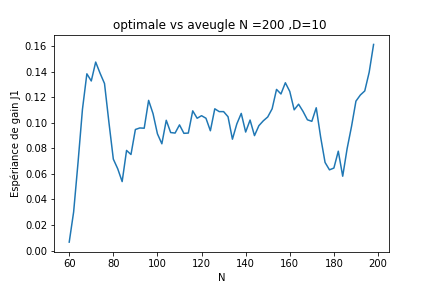
\includegraphics{o_vs_a.png}
\end{center}
Lorsque le joueur 1 choisit le stratégie optimal contre le joueur 2 en choisisant le stratégie aveugle, l'espérance de gain de joueur 1 est proche de 0.11. Le joueur 1 a l'avantage.  

\begin{center}
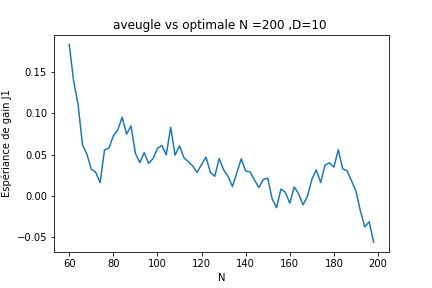
\includegraphics{a_vs_o.png}
\end{center}

Lorsque le joueur 1 choisit le stratégie aveugle contre le joueur 2 en choisisant le stratégie aveugle,plus N est grand l'espérance de gain de joueur 1 est plus petite. Le joueur 2 a l'avantage quand N est assez grand car joueur 1 jouer en premier. 
 
\subsubsection{Question9}
\begin{algorithm}
\caption{Stratégie}
\begin{algorithmic}[1]
\Function{Stratégie aléatoire}{$i$: integer, $j$:integer $D$: integer $N$:integer}
	\State $r$: random vlue between 0 and 1 	
    \State \Return $\lceil r \times D\rceil$ 
\EndFunction
\end{algorithmic}
\end{algorithm}

\section{Variante simultané}
\subsubsection{Question 10}

\begin{equation}\nonumber
EG_{1}(d_{1},d_{2})=\sum\limits_{k1=1}^{6d_{1}}\sum\limits_{k2=1}^{6d_{2}}p(d_{1},k_{1})p(d_{2},k_{2})\frac{\sqrt{(k_{1}-k_{2})^{2}}}{k_{1}-k_{2}}
\end{equation}

la matrice des gains pour D = 3:\\

\begin{tabular}{|c|c|c|c|}
\hline 
\(J_{1} \) - \(J_{2} \) &\(d_{2} \)=1 & \(d_{2} \)=2 &\(d_{2} \)=3\\
\hline  
\(d_{1} \)=1 & 0  &  -0.375  & -0.22685185 \\
\hline 
\(d_{1} \)=2 &  0.375  &  0  &  -0.19881687 \\
\hline 
\(d_{1} \)=3 &  0.22685185  &  0.19881687  &  0 \\
\hline 
\end{tabular}

\subsubsection{Question 11}

si le \(J_{2} \) connait [ \(p_{1}(1)\),  \(p_{1}(2)\),  \(p_{1}(2)\),...,\(p_{1}(D)\)]

si \(J_{2} \) joue j : son expériance de gain est  E(j) = -\(\sum\limits_{i}^{D}EG_{1}(i,j)\)

\begin{equation}\nonumber
\left\{
	\begin{array}{lr}
		p_{2}( \mathop{\arg\max}_{i}(E(j)) ) = 1 & \\
		p_{2}(j) = 0,j\neq\mathop{\arg\max}_{i}(E(j)) 
	\end{array}
\right.
\end{equation}


\subsubsection{Question 12}
\(J_{1} \) doit choisir sa stradégie   [ \(p_{1}(1)\),  \(p_{1}(2)\),  \(p_{1}(2)\),...,\(p_{1}(D)\)] de manière à minimiser la maximum de l'expérience de gain de  \(J_{2} \).
Soit  \(\alpha \)   la maximum de l'expérience de gain de  \(J_{2} \) 
\begin{equation}\nonumber
\left\{
	\begin{array}{lr}
		\min \alpha &\\
			sc\left\{
				\begin{array}{lr}
						\alpha \geq -\sum\limits_{i}^{D}EG_{1}(i,1)p_{1}(i)                   & \\
						\alpha \geq -\sum\limits_{i}^{D}EG_{1}(i,2)p_{1}(i)                   & \\
						...																														& \\
						\alpha \geq -\sum\limits_{i}^{D}EG_{1}(i,D)p_{1}(i)                  & \\
						\sum\limits_{i}^{D}p_{1}(i) = 1																& \\
						p_{1}(1),p_{1}(2),p_{1}(3),...,p_{1}(D) \geq 0
				\end{array}
		\right.
	\end{array}
\right.
\end{equation}


\printindex
\end{document}